% !TEX root = ../../document.tex

\documentclass{subfiles}

\begin{document}

  \chapter{Algoritmos aplicados a Grafos}
  \label{chap:graphs}

    \section{Introducción}
    \label{sec:graphs_intro}

      \paragraph{}
      En las últimas décadas se han dedicado grandes esfuerzos en el estudio de sucesos basados en interelaciones entre elementos. Esto puede entenderse como el análisis de una red de interconexiones modelada como flechas que relacionan un conjunto de puntos. Una gran cantidad de situaciones de la vida cotidiana puede ser representada de esta manera, mediante la cual, se consigue un formalismo matemático enriquecedor sobre el cual resolver distintos problemas que surgen sobre dichas redes.

      \paragraph{}
      Estas redes de interconexiones se pueden apreciar en ámbitos muy dispares, como las ciudades y las carreteras que conectan unas con otras, las personas y las amistades entre si, los teléfonos y las llamadas de unos a otros o las páginas web de internet y los enlaces para navegar de unas a otras. El estudio de estas situaciones es de gran interés en las sociedades modernas, permitiendo una mejora del rendimiento a partir de la extracción de información poco obvia mediante distintas técnicas, lo cual conlleva reducción de costes y un aumento del grado de satisfacción para los usuarios de dichos servicios.

      \paragraph{}
      Sin embargo, utilizar un lenguaje de representación más enriquecedor conlleva sobrecostes asociados que en otros modelos más simples no se dan, lo cual requiere de técnicas sofisticadas para tratar de hacer frente a la resolución de los problemas que se pretende resolver. Además, el crecimiento exponencial en la infraestructura tecnológica ha traido como consecuencia un gran aumento a nivel de tamaño en estos. Algunos ejemplos destacados en el ámbito de internet se dan el protocolo IPv6, que cuenta con $2^128$ posibles direcciones hacia las que poder comunicarse, o el caso de la red social \emph{Facebook}, que cuenta con 1 trillón de relaciones de amistad, tal y como se indica en \emph{One trillion edges: Graph processing at facebook-scale} \cite{ching2015one}.

      \paragraph{}
      Conforme el tamaño de las redes aumenta, una estrategia razonable es la de utilizar soluciones aproximadas para la resolución de los problemas que se plantean sobre ellas, a través de los cuales se pretende encontrar una solución cercana a la exacta (admitiendo una desviación máxima de $\epsilon$, que se cumple con probabilidad $\delta$), lo que otorga como ventaja una reducción significativa tanto desde la perspectiva del coste temporal como del espacial en la resolución del problema.

      \paragraph{}
      En este capítulo se pretende realizar una descripción acerca de las distintas alternativas posibles para tratar de agilizar la resolución de problemas sobre redes de tamaño masivo utilizando técnicas aproximadas. Por tanto, primero se ha realizado una descripción formal sobre el modelo de representación de grafos en la sección \ref{sec:graph_formalism}. A continuación, se ha descrito un modelo sobre el cual diseñar algoritmos que resuelvan problemas aplicados a grafos tratando de aprovechar al máximo el espacio en memoria (que se considera limitada) y reduciendo el número de accesos sobre el espacio de almacenamiento mediante el \emph{modelo en semi-streaming}, del cual se habla en la sección \ref{sec:semi_streaming_model}. El siguiente tema que se trata en este capítulo se refiere a técnicas que tratan de reducir la complejidad de una red de tamaño masivo mediante la eliminación de relaciones entre sus punto mediante la utilización de \emph{Spanners} y \emph{Sparsifiers} en la sección \ref{sec:spanners_sparsifiers}. Después, se ha realizado una breve descripción acerca de distintos problemas bien conocidos para los cuales se han encontrados soluciones sobre el \emph{modelo en semi-streaming} en la sección \ref{sec:graph_problems}. Finalmente se ha realiza una breve conclusión en la sección \ref{sec:graph_conclusions}.

    \section{Definición Formal}
    \label{sec:graph_formalism}

      \paragraph{}
      En esta sección se describen los conceptos básicos necesarios para entender el estudio de problemas modelados como \emph{Grafos}. Para la descripción formal sobre dichas estructuras se han utilizado las notas de clase de la asignatura de \emph{Matemática Discreta} \cite{matematicaDiscreta2016notes} impartida en la \emph{Universidad de Valladolid} así como las de la asignatura equivalente (\emph{Discrete Mathematics CS 202} \cite{aspnes2013notes}) impartida por \emph{Aspnes} en la \emph{Universidad de Yale}.

      \paragraph{}
      La \textbf{Teoría de Grafos} (\emph{Graph Theory}) es la disciplina encargada del estudio de estructuras compuestas por vértices y aristas desde una persepectiva matemática. Los vértices representan objetos o elementos, mientras que las aristas se corresponden con las relaciones que se dan entre vértices. Un grafo $G$ se define por tanto como la tupla del conjunto de vértices $V = \{ v_1, _2, ..., v_n \}$ y el conjunto de aristas $E = \{ e_1, e_2, ..., e_m \}$, de tal manera que $e_j = (v_{i_1}, v_{i_2})$ representa el arista que conecta el vértice $v_{i_1}$ con el vértice $v_{i_2}$. Nótese por tanto, que el grafo está compuesto por $n$ vértices y $m$ aristas. El grafo $G$ se puede modelizar por tanto como $G = (V, E)$. En la figura \ref{img:graph_example} se muestra una representación gráfica de un determinado grafo no dirigido compuesto por $6$ vértices y $7$ aristas.

      \begin{figure}
        \centering
        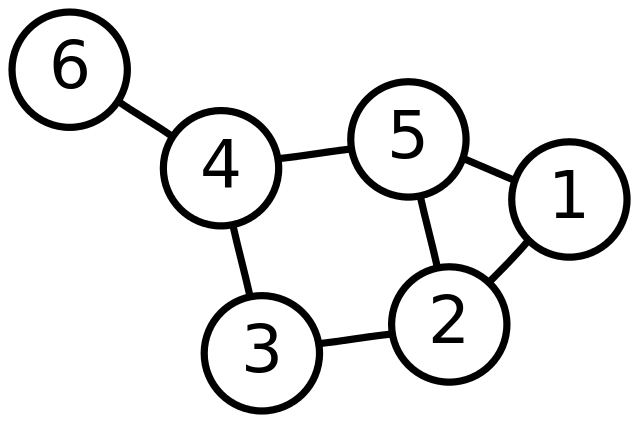
\includegraphics[width=0.4\textwidth]{graph-example}
        \caption{Ejemplo de \emph{Grafo No Dirigido}. (Extraido de \cite{wiki:Graph_(discrete_mathematics)})}
        \label{img:graph_example}
      \end{figure}

      \paragraph{}
      Aquellos grafos para los cuales la arista $e_j$ representa los dos sentidos de la relación, es decir, $v_{i_1}$ está relacionado con $v_{i_2}$ y $v_{i_2}$ está relacionado con $v_{i_1}$ se denominan \emph{Grafos no nirigidos}, mientras que en los casos en que esta relación no es recíproca se habla de \emph{Grafos dirigidos}. Cuando cada arista $e_j$ tiene asociado un determinado peso $w_j \in W =  \{ w_1, w_2, ..., w_m\}$ se dice entonces que $G$ es un \emph{grafo ponderado} y se denota como $G=(V, E, W)$, mientras que cuando se presupone que todas las aristas tienen el mismo peso $W$ se omite de la notación.

      \paragraph{}
      Cuando un vértice denominado $v_{i_1} \in V$ está directamente relacionado con otro $v_{i_2} \in V$, es decir, existe una arista $e_j \in E$ que los conecta ($e_j = (v_{i_1}, v_{i_2})$) se dice que son $e_j$ es \emph{incidente} sobre dichos vértices. De la misma manera se dice que $v_{i_1}$ y $v_{i_2}$ son \emph{adjacentes} entre sí.

      \paragraph{}
      Respecto del conjunto de aristas incidentes sobre cada vértice, se denomina \emph{grado} al cardinal dicho conjunto, diferenciando en los grafos no dirigidos entre \emph{in-grado} a las de entrada y \emph{out-grado} a las de salida. Se utiliza la notación $d(v_i)$ para referirse al grado del vértice i-ésimo, $d^+(v_i)$ al \emph{in-grado} y $d^-(v_i)$ al \emph{out-grado} de dicho vértice. Nótese por tanto, que se cumple la siguiente propiedad: $d(v_i) = d^+(v_i) + d^-(v_i)$.


      \paragraph{}
      Un \emph{camino} es un conjunto de aristas $P_p = \{ e_{k_1}, e_{k_2}, ..., e_{k_p}\}$, tales que el arista k-ésimo tiene como vértice de destino el mísmo que utiliza el arista $k+1$ como vércice origen. Nótese que el valor $p$ indica la \emph{longitud} del camino. Cuando el vértice de destino de la arista $e_{k_p}$ es el mismo que el de origen de $e_{k_1}$ se denomina \emph{ciclo} y se denomina $C_p$.

      \paragraph{}
      Se denota como $K_n$ al grafo compuesto por $n$ vértices y $n*(n-1)$ aristas, de tal manera que estas conectan cada vértice con todos los demás. Los grafos que cumplen esta propiedad se denominan grafos completos de grado $n$. Nótese que el cardinal de aristas se reduce a la mitad en el caso de los grafos no dirigidos.

      \paragraph{}
      Cuando al estudiar la estructura de un grafo, se comprueba que el conjunto de vértices puede dividirse en dos subconjuntos disjuntos $V_1$ y $V_2$, de tal manera que para todas las aristas $e_j = (v_{i_1}, v_{i_2})$ el vértice $v_{i_1}$ se encuentra en el subconjunto $V_1$ y el vértice $v_{i_2}$ se encuentra en el subconjunto $V_2$, entonces se habla de un \emph{Grafo Bipartito}. Un ejemplo de esta situación se muestra en la figura \ref{img:bipartite_graph_example}. Nótese que el concepto de grafo bipartito puede extenderse fácilmente a más de dos subconjuntos, denominandose entonces \emph{Grafo k-partito}. Estos grafos son de gran utilidad para modelizar algunos problemas tales como los que se dan en empresas como \emph{Netflix}, para los cuales $V_1$ puede estar formado por el conjunto de usuarios mientras que $V_2$ representa el contenido multimendia. Por tanto, cada arista puede entenderse como una visualización del usuario $v_{i_1} \in V_1$ sobre el contenido $v_{i_2} \in V_2$ .

      \begin{figure}
        \centering
        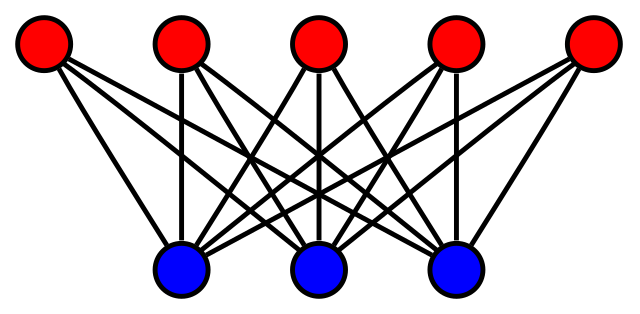
\includegraphics[width=0.4\textwidth]{bipartite-graph-example}
        \caption{Ejemplo de \emph{Grafo Bipartito}. (Extraido de \cite{wiki:Graph_(discrete_mathematics)})}
        \label{img:bipartite_graph_example}
      \end{figure}

      \paragraph{}
      Un \emph{subgrafo} $H$ es el grafo compuesto por un subconjunto de vectores y aristas del grafo $G$. Nótese que en el caso de que se eliminen vértices, es necesario eliminar también todas sus aristas incidentes. Esto se puede indicar de manera matemática de la siguiente forma: $H \subseteq G$ por lo que $H_V \subseteq G_V$ y $H_E \subseteq G_E$.

      \paragraph{}
      Desde el punto de vista de las transformaciones que se pueden realizar sobre grafos, se denomina \emph{isomorfismo} a una transformación biyectiva sobre el grafo $G =(V_G, E_G)$ al grafo $H = (V_H, E_H)$ que se realiza sobre los vértices de manera que $f: V_G \rightarrow V_H$ y por cada arista $(e_1, e_2) \in E_G$, entonces $(f(e_1), f(e_2)) \in E_H$ de tal manera que la estructura de $G$ se conserva en $H$. Entonces se dice que $G$ y $H$ son isomorfos entre si. Si se modifica la condición de biyectividad del \emph{isomorfismo} y tan solo se requiere la propiedad de inyectividad entonces se habla de \emph{homomorfismo}. Por tanto, esto puede ser visto como una transformación sobre la cual no se mantiene la estructura de $G$, entonces $H$ ya no es equivalente a $G$, sino que es un \emph{subgrafo} de este.

      \paragraph{}
      Las transformaciones son interesantes desde el punto de vista del tratamiento de grafos de tamaño masivo, dado que a partir de estas se trata de reducir la complejidad cuando el tamaño de estos los hace intratables. Por lo tanto, en este caso interesa conseguir transformaciones que reduzcan el tamaño del grafo, pero que tratan de mantener su estructura lo más semejante posible. Destacan transformaciones conocidas como \emph{Spanners} (de los que se hablará en la sección \ref{sec:spanners}) y \emph{Sparsifiers} (en la sección \ref{sec:sparsifiers}).

      \subsection{Métodos de Representación}
      \label{sec:representation_methods}

        \paragraph{}
        Existen diversas estrategias para representar un grafo sobre estructuras de datos, las cuales presentan distintas ventajas e inconvenientes, tanto a nivel de espacio como de tiempo de acceso. Dichas estrategias se escogen teniendo en cuenta la estructura del grafo. En esta sección se habla de matrices de adyacencia, de listas de adyacencia y de la matriz laplaciana, la cual contiene un conjunto de propiedades interesantes que pueden ser muy útiles en la resolución de algunos problemas.

        \subsubsection{Matriz de Adyacencia}
        \label{sec:adjacency_matrix}

          \paragraph{}
          Se denomina matriz de adyacencia $A$ del grafo $G = (V,E)$ compuesto por $n=|V|$ vértices, $m=|E|$ aristas y $W$ el conjunto de pesos de los aristas a una matriz de tamaño $n*n$ construida tal y como se indica en la ecuación \eqref{eq:adjacency_matrix}. Nótese que esta definición es válida tanto para grafos ponderados como para no ponderados suponiendo que $w_k = 1, k \in [1, m]$.

          \begin{equation}
          \label{eq:adjacency_matrix}
            A_{i,j} =
              \begin{cases}
                w_k,  & (v_i, v_j) = e_k \in E\\
                0,    &\text{en otro caso}
              \end{cases}
          \end{equation}

          \paragraph{}
          Esta estrategia de representación es apropiada cuando se trabaja sobre grafos altamente conexos (con un gran número de aristas), ya que el número de posiciones nulas en la matriz es reducido y la estructura matricial indexada proporciona un tiempo de acceso de $O(1)$ a cada posición. Sin embargo, se requiere de $O(n^2)$ para almacenar dicha matriz, algo admisible cuando $n^2 \approx m$ para lo que esta representación se acerca a su óptimo espacial.

        \subsubsection{Lista de Adyacencia}
        \label{sec:adjacency_list}

          \paragraph{}
          La alternativa a la codificación del grafo como una matriz de adyacencia se conoce como \emph{lista de adyacencia}. En este caso, se mantiene una lista (posiblemente ordenada u otras estrategias estructuradas como listas enlazadas o árboles, para tratar de reducir los tiempos de acceso) para almacenar el conjunto de aristas $E$. Nótese por tanto, que en este caso la codificación es óptima a nivel de espacio $O(m)$, no existiendo una estrategia de representación que pueda almacenar la estructura del mismo de manera exacta utilizando un tamaño menor. Sin embargo, tal y como se puede intuir, el tiempo de acceso es de $O(m)$ en el peor caso. Esta solución es apropiada para grafos muy dispersos (aquellos en que $n \ll m$).

        \subsubsection{Matriz Laplaciana}
        \label{sec:laplacian_matrix}

          \paragraph{}
          La \emph{matriz laplaciana} consiste en una estrategia de representación de grafos que cumple importantes propiedades, a partir de las cuales se facilita en gran medida la resolución de distintos problemas, entre los que se encuentran \emph{árboles de recubrimiento} (sección \ref{sec:minimum_spanning_tree}), aunque también se utiliza en la estimación de la distribución de probabilidad de \emph{paseos aleatorios} (sección \ref{sec:random_walks_overview}).

          \paragraph{}
          El método de construcción de la \emph{matriz laplaciana} se indica en la ecuación \eqref{eq:laplacian_matrix}, el cual genera una matriz $L$ de tamaño $n * n$ (al igual que en el caso de la matriz de adjacencia) que aporta información sobre el grafo subyacente. La diagonal de la matriz laplaciana contiene el grado del vértice referido a dicha posición, mientras que el resto de las celdas se construyen colocando el valor $-w_k$ cuando existe un arista entre el vértice $v_i$ y el vértice $v_j$ ( $e_k = (v_i,v_j) \in E$ ) y $0$ cuando no existe. La matriz laplaciana también puede entenderse como $L = D - A$ donde $D$ representa una matriz diagonal de tamaño $n*n$ que almacena el grado del vértice $v_i$ en la posición $D_{i,i}$ y $0$ en otro caso, mientras que $A$ se corresponde con la matriz de adyacencia descrita anteriormente.

          \begin{align}
          \label{eq:laplacian_matrix}
            L_{{i,j}} = {\begin{cases}
              d(v_{i})&{\mbox{if}}\ i=j\\
              -1&{\mbox{if}}\ i\neq j\ {\mbox{and}}\ v_{i}{\mbox{ is adjacent to }}v_{j}\\
              0&{\mbox{otherwise}}\end{cases}}
          \end{align}

          \paragraph{}
          A partir de esta representación se facilita la resolución de distintos problemas tal y como se ha indicado anteriormente. También existen distintas variaciones respecto de la descrita en esta sección, entre las que se encuentran la \emph{matriz laplaciana normalizada} o la \emph{matriz laplaciana de caminos aleatorios}, de la cual se hablará en el capítulo \ref{chap:pagerank} para el cálculo del ranking de importancia \emph{PageRank}.


      \paragraph{}
      En la práctica, cuando se trabaja con grafos de tamaño masivo, es muy común que estos sean muy dispersos. Algunos ejemplos de ello son el \emph{grafo de la web} (grafo dirigido), en el cual cada vértice representa sitio web y cada arista un enlace hacia otro sitio web. Es fácil comprobar que este grafo es altamente disperso ya que es muy poco probable que un sitio web contenga enlaces al resto de sitios de la red cuando se habla de millones de vértices. Algo similar ocurre en el caso de redes sociales como \emph{Facebook} (grafo no dirigido debido a relaciones de amistad) o \emph{Twitter} (grafo dirigido debido a relaciones seguimiento). Por tanto, la representación mediante listas de adyacencia es una herramienta útil a nivel conceptual pero que en la práctica no se utiliza por la inviabilidad derivada del gran coste espacial para su almacenamiento.

    \section{Modelo en Semi-Streaming}
    \label{sec:semi_streaming_model}

      \paragraph{}
      Al igual que sucede en el caso de conjuntos de datos de carácter numérico y categoríco, en el modelo de grafos, también es necesario hacer frente al elevado tamaño del problema mediante nuevas estrategias de diseño de algoritmos. El \emph{modelo en streaming}, del cual se habló en la sección \ref{sec:streaming_model} es una buena alternativa para tratar de agilizar la búsqueda de soluciones que varían con respecto del tiempo, además de trabajar sobre un espacio reducido lo cual aprovecha en mayor medida las capacidades del hardware subyacente. Tal y como se indicó anteriormente, esta estrategia permite reducir el número de acceso sobre el dispositivo de almacenamiento tratando de trabajar únicamente con los estimadores que se mantienen en la memoria del sistema, cuyo tiempo de acceso es mucho más redudido.

      \paragraph{}
      Sin embargo, en el caso de los problemas referidos a grafos, este modelo presenta mayores dificultades, tanto a nivel de espacio como del número de accesos sobre el stream de datos por la estructura enlazada de la representación de grafos. Por lo tanto, se han definido variaciones sobre el \emph{modelo en streaming} original para tratar de hacer frente a los requisitos característicos de este tipo de problemas. En los artículos \emph{On graph problems in a semi-streaming model} \cite{feigenbaum2005graph} y \emph{Analyzing graph structure via linear measurements} \cite{ahn2012analyzing} los autores describen dicho modelo, al cual denominan \textbf{Modelo en Semi-Streaming}.

      \paragraph{}
      Este se corresponde con una relajación del \emph{modelo en streaming} estándar, el cual permite mayor libertad tanto a nivel de espacio como de pasadas permitidas sobre el stream de datos. Por esta razón, cuando el número de pasadas $p$ es superior a 1 ($p > 1$), entonces ya no es posible su uso en entornos en que se requiere que el procesamiento de la información y las consultas sean en tiempo real, algo que, por contra, si sucedía en el caso del \emph{modelo en streaming} definido anteriormente. Por lo tanto, el \emph{modelo en semi-streaming} se presenta como una estrategia de diseño de algoritmos que trata de obtener estimaciones sobre grafos en un espacio reducido y con un buen planteamiento a nivel de accesos a disco cuando el grafo completo no puede mantenerse en la memoria del sistema de manera completa.

      \paragraph{}
      El \emph{modelo en semi-streaming} impone la forma en que el grafo es recibido bajo la idea de stream de datos, lo cual se describe a continuación: Sea $G = (V, E)$ un grafo dirigido (su adaptación al caso de grafos no dirigidos es trivial) compuesto por $n = |V|$ vértices y un número indeterminado de arístas desde el punto de vista del algoritmo que procesará el stream. Se presupone que se conoce \emph{a-priori} el número de vértices que forman el grafo, mientras que el stream consiste en el conjunto de tuplas que representan las aristas. El conjunto de aristas $E$ se define como $E = \{ e_{i_1}, e_{i_2}, ..., e_{i_j}, ..., e_{i_m} \}$, tal y como se ha hecho en secciones anteriores. Por tanto el grafo $G$ está formado por $m = |E|$ aristas (es necesario remarcar que el algoritmo que procesa el stream no conoce dicho valor). Dichas aristas son procesadas en un orden desconocido de manera secuencial marcado por el conjunto de permutaciones arbitrarias $\{ i_1, i_2, i_j, i_m \}$ sobre $[1, m]$.

      \paragraph{}
      Una vez descrita la estrategia de procesamiento sobre el \emph{modelo en semi-streaming}, lo siguiente es indicar las unidades de medida sobre las cuales realizar el análisis sobre la complejidad de los algoritmos que se desarrollan sobre este modelo. En \cite{feigenbaum2005graph}, los autores definen $S(n,m)$ como el espacio utilizado para procesar el stream de aristas, $P(n,m)$ el número de pasadas sobre dicho stream y $T(n,m)$ el tiempo necesario para procesar cada arista. Sobre esta contextualización se requiere que para que un algoritmo sea válido en el \emph{modelo en semi-streaming} $S(n,m)$ esté contenido en el orden de complejidad $O(n \cdot polylog(n))$. Tal y como se puede apreciar, esta restrición a nivel de espacio es mucho más relajada que la impuesta sobre el \emph{modelo en streaming} estándar, que requiere de $o(N)$. Sin embargo, es necesario tener en cuenta que gran cantidad de problemas sobre grafos requieren un coste espacial de $O(n^2)$, por lo que tratar de encontrar una solución en $O(n \cdot polylog(n))$ representa una tarea compleja, pero conlleva una mejora significativa.

      \paragraph{}
      Al igual que sucede con en el caso del \emph{modelo en streaming} estándar, al utilizar un orden espacial menor del necesario para encontrar soluciones exactas, las soluciones encontradas admiten la existencia de una determinada tasa de error máxima delimitada por $\epsilon$, la cual se debe cumplir con una probabilidad $\delta$. Para conjuntos de datos sobre los cuales no es admisible la búsqueda de una solución exacta o para los cuales sea admisible una reducida tasa de error, esta estrategia de diseño de algoritmos se presenta por tanto como una alternativa acertada.

    \section{Spanners y Sparsifiers}
    \label{sec:spanners_sparsifiers}

      \paragraph{}
      Para tratar de agilizar los cálculos necesarios para la resolución de problemas sobre grafos, se han propuesto distintas alternativas, muchas de las cuales son aplicables únicamente a problemas concretos. Sin embargo, estas ideas se discutirán en la sección \ref{sec:graph_problems}. En esta sección se describen distintas técnicas utilizadas para tratar de \say{sumarizar} o disminuir el espacio necesario para almacenar un determinado grafo $G$ (al igual que ocurría con las técnicas descritas en el capítulo anterior para valores numéricos) transformándolo en un nuevo grafo $H$, de tal manera que la estructura del mismo siga siendo lo más similar a la del original respecto de distintas medidas.

      \paragraph{}
      La descripción de estas técnicas se ha basado en las ideas recogidas en los artículos \emph{Graph stream algorithms: a survey} \cite{mcgregor2014graph} de \emph{McGregor} y \emph{Graph sketches: sparsification, spanners, and subgraphs} \cite{ahn2012graph} de \emph{Ahn y otros}, así como las notas de la \emph{Clase 11} de la asignatura \emph{Randomized Algorithms} \cite{harvey2011randomized} impartida en la \emph{Universidad de Columbia Británica}. Tal y como se ha indicado en el párrafo anterior, estas técnicas consisten en la eliminación de vértices y/o aristas, de tal manera que la distorsión producida tras dichas modificaciones sea mínima.

      \paragraph{}
      Existe un enfoque trivial para la reducción del tamaño en grafos, sin embargo, este tan solo ofrece resultados aceptables sobre grafos densos (aquellos similares al grafo completo $K_n$). La técnica consiste en la eliminación de aristas a partir de una determinada tasa de probabilidad $\alpha$. Mediante esta estrategia se reduce el espacio necesario para almacenar las aristas de $(1-\alpha)$. Tal y como se ha dicho, esta solución tan solo es válida en aquellos casos en que el grafo sea denso. Cuando el grafo es disperso, por contra, la eliminación de aristas mediante la selección uniforme puede producir una gran distorsión respecto del grafo original.

      \begin{figure}
        \centering
        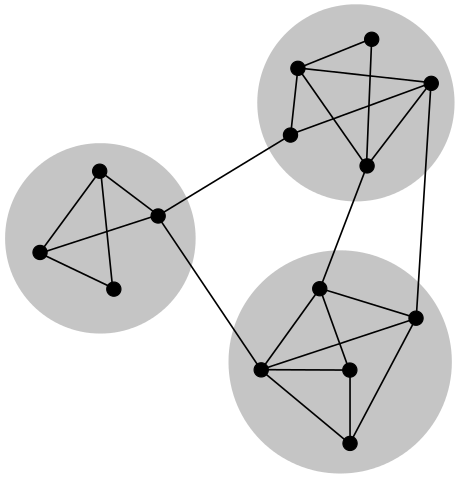
\includegraphics[width=0.3\textwidth]{graph-community-structure}
        \caption{Ejemplo de \emph{Grafo Disperso}. (Extraido de \cite{wiki:Community_structure})}
        \label{img:graph_community_structure}
      \end{figure}

      \paragraph{}
      En la figura \ref{img:graph_community_structure} se muestra un grafo disperso, que además forma 3 comunidades (conjuntos de vértices altamente conexos entre sí). Nótese que en aquiellos casos en que el grafo posea una estructura similar a la del de la figura, ya no es conveniente utilizar la estrategia descrita en el párrafo anterior, puesto que para tratar de preservar la estructura del mismo, no todas las aristas tienen la misma relevancia. Esto puede entenderse de manera sencilla si al comprobar la variación del grafo al eliminar una de las aristas que conectan dos comunidades. Dicha variación estructural es significativamente mayor que la ocurrida tras eliminar una arista que conecta dos vértices pertenecientes a una misma comunidad.

      \paragraph{}
      Por esta razón, distintos autores han trabajado en técnicas para tratar de mantener la estructura del subgrafo generado lo más semejante posible a la del grafo original. Para ello, las estrategias más populares se basan en la utilización de \emph{Spanners} y \emph{Sparsifiers}, los cuales se describirán a continuación en las secciones \ref{sec:spanners} y \ref{sec:sparsifiers} respectivamente. Estas técnicas han sido ampliamente estudiadas, sin embargo, en este caso se pretende orientar la descripción de las mismas sobre el \emph{modelo en semi-streaming} del cual se habló anteriormente. En este modelo se han encontrado soluciones eficientes para \emph{grafos no dirigidos}. Por contra, para el caso de los \emph{grafos dirigidos}, la búsqueda de soluciones eficientes para este problema continua siendo un problema abierto.

      \subsection{Spanners}
      \label{sec:spanners}

        \paragraph{}
        Se denomina \emph{Spanner} a un determinado subgrafo que mantiene las propiedades de distancia entre todos sus vértices respecto del original con una tasa máxima de variación acotada por $\alpha$. Por tanto, se denomina \emph{$\alpha$-spanner} del grafo $G = (V, E)$ a un subgrafo $H = (V, E')$ donde $E' \subset E$, construido de tal manera que se cumpla la ecuación \eqref{eq:alpha_spanner} representando $d_G(v_{i_1},v_{i_2})$ la distancia del camino más corto entre los vértices $v_{i_1}$ y $v_{i_2}$ sobre el grafo $G$.

        \begin{equation}
        \label{eq:alpha_spanner}
          \forall v_{i_1}, v_{i_2} \in V, \ d_G(v_{i_1},v_{i_2}) \leq d_H(v_{i_1},v_{i_2}) \leq \alpha \cdot d_G(v_{i_1},v_{i_2})
        \end{equation}

        \paragraph{}
        Tal y como se indica en la ecuación \eqref{eq:alpha_spanner}, lo que se pretende acotar mediante esta estrategia es, por tanto, el error desde el punto de vista de la distancia entre vértices. Tal y como se puede intuir, mediante el cumplimiento de esta propiedad se soluciona el problema descrito anteriormente que surge sobre grafos dispersos, dado que si se elimina el único arista que conecta dos comunidades distintas, entonces la distancia del camino más corto entre los vértices de comunidades distintas variará en gran medida, posiblemente superando la acotada del valor $\alpha$.

        \paragraph{}
        Para la construcción de un \emph{$\alpha$-spanner} sobre el modelo en streaming existe un algoritmo sencillo que resuelve este problema para el caso del modelo de caja registradora (sección \ref{sec:streaming_cash_register}), es decir, en el cual tan solo estén permitadas adicciones. Esta estrategia se ilustra en el algoritmo \ref{code:basic_spanner}. En este caso, la solución es trivial y consiste en añadir únicamente al conjunto de aristas $E'$ del grafo $H$, aquellas cuya distancia del camino más corto entre sus vértices en $H$ sea mayor que $\alpha$, con lo cual se garantiza la propiedad del \emph{$\alpha$-spanner}.

        \paragraph{}
        \begin{algorithm}
          \SetAlgoLined
          \KwResult{$E'$ }
          $E' \gets \emptyset$\;
          \For{cada $(u, v) \in E$}{
            \If{$d_H(u,v) > \alpha$}{
              $E' \gets E' \cup \{(u,v)\}$\;
            }
          }
          \caption{Basic Spanner}
          \label{code:basic_spanner}
        \end{algorithm}

        \paragraph{}
        Sin embargo, esta técnica requiere del cálculo del camino más corto entre los vértices $u$ y $v$ en cada actualización, lo cual genera un coste de $O(card(E'))$ en tiempo, o el mantenimiento de una estructura de datos auxiliar que almacene dichas distancias, lo que requiere de un $O(n^2)$ en espacio. El mejor resultado encontrado para este problema es la construcción de un \emph{$(2k-1)$-spanner} utilizando $O(n^(1+1/k)$ de espacio. Esta solución se ha demostrado que es óptima respecto de la precisión utilizando tan solo una pasada sobre el stream de aristas. La descripción completa de la misma se encuentra en el trabajo \emph{Streaming and Fully Dynamic Centralized Algorithms for Constructing and Maintaining Sparse Spanners} \cite{elkin2007streaming} de \emph{Elkin}.

        \paragraph{}
        Para el caso general, en el cual están permitidas tanto adicciones como eliminaciones (modelo en molinete descrito en la sección \ref{sec:streaming_turnstile}) la solución básica no es trivial. El algoritmo que se describe en \cite{elkin2007streaming} se basa en la generación de árboles incrementales que se construyen a partir de la selección aleatoria de vértices. Sin embargo, esto no es sencillo cuando se permiten las eliminaciones. Por lo tanto, para la adaptación de dichas técnicas al modelo en molinete una solución es la utilización de \emph{$L_0$-Samplers}, que se describieron en la sección \ref{sec:lp_samplers}, lo que requiere de múltiples pasadas sobre el stream de aristas.

        \paragraph{}
        Tal y como se ha visto en esta sección, la construcción de \emph{Spanners} añade un sobrecoste a la resolución de problemas sobre grafos, junto con una determinada tasa de error desde el punto de vista de la distancia entre vértices. Sin embargo, dichos inconvenientes se ven recompensados en muchos casos por la reducción en tiempo y espacio de la resolución del problema sobre el subgrafo resultante.

      \subsection{Sparsifiers}
      \label{sec:sparsifiers}

        \paragraph{}
        Otra alternativa para la generación del subgrafo $H$ construido sobre el mismo conjunto de vértices y un subconjunto de aristas respecto del grafo $G$ son los \emph{Sparsifiers}. En este caso, en lugar de tratar de mantener la propiedad de la distancia del camino más corto entre pares de vértices, se basa en la minimización del número de cortes mínimos (eliminación de aristas) para separar el conjunto de vértices del grafo en dos subconjuntos disjuntos para cada par de vértices. A este concepto se lo denomina \emph{corte mínimo} (o \emph{Minimun Cut}) y se denota por $\lambda_{u,v}(G)$ para indicar el número de aristas a eliminar para formar dos subconjuntos disjuntos $V_{1}, V_{2}$ de tal manera que $u\in V_{1}$ y $v \in V_{2}$. Nótese por tanto, que en un grafo dirigido el \emph{corte mínimo} puede tomar valores en el intervalo $[1, n\cdot(n-1)]$.  En la ecuación \eqref{eq:sparsifier_cut} se muestra la definición formal de \emph{Sparsifier} donde $A$ representa todas las combinaciones de pares de vértices y $\epsilon$ la desviación máxima permitida por el \emph{Sparsifier}, de tal manera que el resultado se corresponde con un \emph{$(1 +\epsilon)$-Sparsifier}.

        \begin{figure}
          \centering
          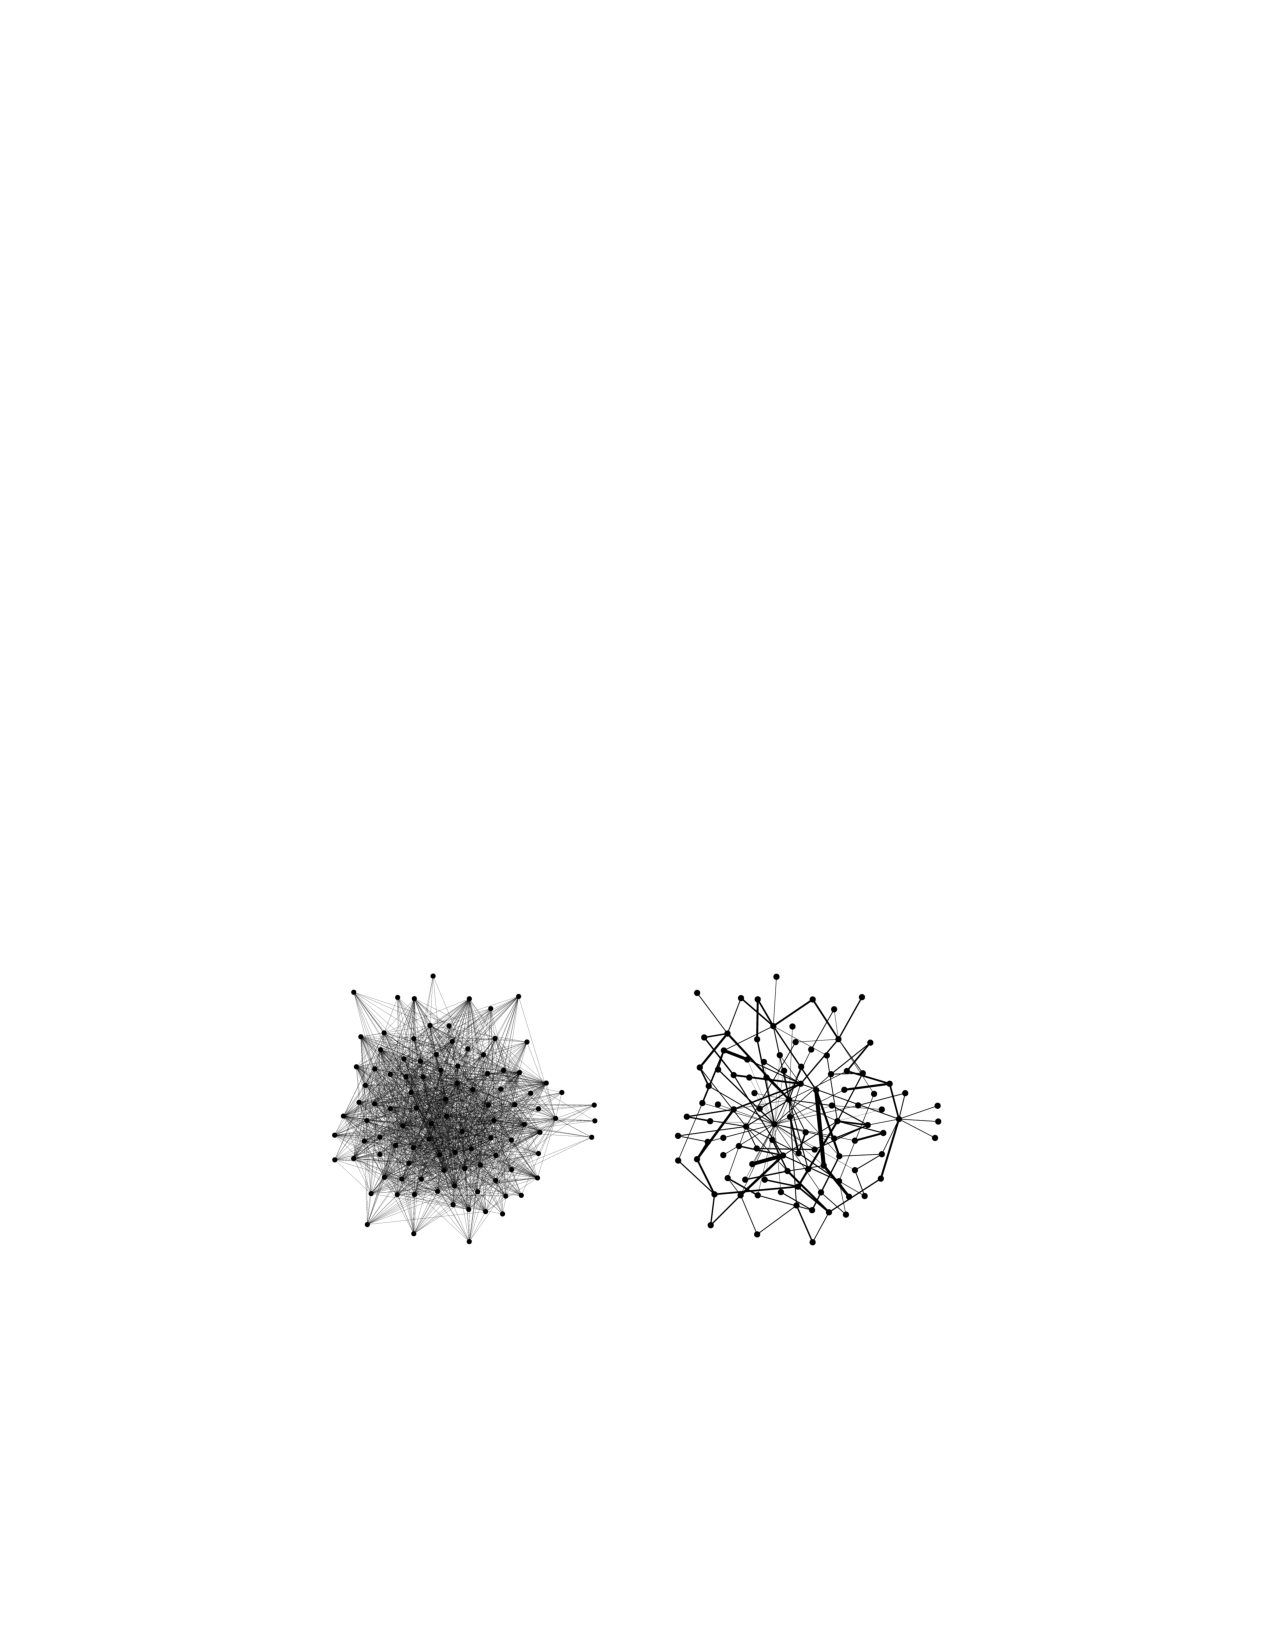
\includegraphics[width=0.5\textwidth]{graph-sparsifier}
          \caption{Ejemplo de \emph{Sparsifier}. (Extraido de \cite{harvey2011randomized})}
          \label{img:graph_community_structure}
        \end{figure}

        \begin{equation}
        \label{eq:sparsifier_cut}
          \forall A \in V \  (1-\epsilon)\lambda_A(G)\leq\lambda_A(H)\leq(1+\epsilon)\lambda_A(G)
        \end{equation}

        \paragraph{}
        A continuación se describe una definición para entender las ideas subyacentes en que se basan los \emph{Sparsifiers}. Para construir un \emph{$(1 +\epsilon)$-Sparsifier} de $G$, el valor $p$ debe ser escogido tal y como se indica en la ecuación \eqref{eq:sparsifier_p} donde $\lambda(G)$ representa el corte mínimo de $G$. La demostración se encuentra en el artículo \emph{On graph problems in a semi-streaming model} \cite{feigenbaum2005graph} desarrollado por \emph{Feigenbaum y otros}. Por tanto, el problema se reduce al mantenimiento de un \emph{$L_{0}$-Sampler} que devuelva un subconjunto de aristas seleccionados con probabilidad $p$ del stream de aristas.

        \begin{equation}
        \label{eq:sparsifier_p}
          p \geq min\{6\lambda(G)^{-1}\epsilon^{-2}log(n),1\}
        \end{equation}

        \paragraph{}
        A continuación se describe una estrategia sencilla de construcción de \emph{$(1 +\epsilon)$-Sparsifiers} para grafos no dirigidos. Esta se basa en la selección de aristas con probabilidad $p$ definido tal y como se indicó anteriormente en la ecuación \eqref{eq:sparsifier_p}.

        \paragraph{}
        \begin{algorithm}
          \SetAlgoLined
          \KwResult{$E'$ }
          $E' \gets \emptyset$\;
          \For{cada $(u, v) \in E$}{
            $r \gets Uniform(0,1)\;$ \\
            \If{$r < p$}{
              $E' \gets E' \cup \{(u,v)\}$\;
            }
          }
          \caption{Basic Sparsifier}
          \label{code:basic_sparsifier}
        \end{algorithm}

        \paragraph{}
        Otro enfoque más general para la construcción de \emph{Sparsifiers} se basa en la utilización de la \emph{Matriz Laplaciana} (definida en la sección \ref{sec:laplacian_matrix}) del grafo $H$, que denotaremos como $L_{H}$. A los \emph{Sparsifiers} construidos manteniendo la propiedad definida en la ecuación \eqref{eq:sparsifier_spectral} se los denomina \emph{Spectral Sparsifiers}. Desarollando la ecuación obtenida si restringimos el rango de valores de $x$ al subconjunto $\{ 0, 1\}^n$ entonces podemos obtener la ecuación \ref{eq:sparsifier_cut}. Dado que el vector $x$ modeliza el conjunto $A$ en dicha ecuación. Por tanto, los \emph{Spectral Sparsifiers} pueden ser vistos como una generalización de los anteriores.

        \begin{equation}
        \label{eq:sparsifier_spectral}
          \forall x \in \mathbb{R} \leq (1 - \epsilon) x^TL_{G}x \leq x^TL_{H}x \leq (1 + \epsilon) x^TL_{G}x
        \end{equation}

        \paragraph{}
        Mediante la estrategia de los \emph{Spectral Sparsifiers}, además de aproximar el corte mínimo $\lambda(G)$ se pueden aproximar otras propiedades como propiedades de los paseos aleatorios (que se describen en la sección \ref{sec:random_walks_overview}). En el trabajo \emph{Twice-Ramanujan Sparsifiers} \cite{batson2012twice} redactado por \emph{Batson y otros} se describe una estrategia de construcción de \emph{$(1 +\epsilon)$-Spectral Sparsifiers} en un espacio de $O(\epsilon^{-2}n)$.

        \paragraph{}
        [TODO ampliar sección]

        \paragraph{}
        [TODO ampliar sección]

        \paragraph{}
        [TODO ampliar sección]

      \paragraph{}
      Las estrategias descritas en esta sección para la reducción de la complejidad de grafos ajustandose al \emph{modelo en semi-streaming} proporcionan una ventaja significativa a nivel de espacio mediante la redución del conjunto de aristas para la resolución de otros problemas a partir de ellas. Por contra, estas generan una determinada tasa de error.

      \paragraph{}
      Cuando se ha hablado de optimalidad en esta sección, ha sido desde el punto de vista de los \emph{grafos no dirigidos}, dado que para el caso de los \emph{grafos dirigidos}, aún no se han encontrado métodos de generación de \emph{Spanners} o \emph{Sparsifiers} óptimos debido a la mayor complejidad que estos conllevan. En la siguiente sección se describen distintos problemas para los cuales se ha encontrado una solución sobre el \emph{modelo en semi-streaming} y sus correspondientes restricciónes.

    \section{Problemas sobre Grafos}
    \label{sec:graph_problems}

      \paragraph{}
      El modelo de representación de grafos proporciona un marco de trabajo flexible sobre el cual se pueden modelizar un gran número de situaciones. Un ejemplo característico de esta situación son las redes sociales, en las cuales cada persona representa un vértice en el grafo mientras que las aristas representan las relaciones entre estas. El conjunto de relaciones generadas a partir de los enlaces entre páginas web (\emph{Web Graph}) también son un claro ejemplo de problemas que se pueden representar mediante un grafo. Sin embargo, este modelo permite representar otras muchas situaciones como planificación de tareas donde cada vértice representa una tarea y las aristas marcan el orden de precedencia de las mismas. Los grafos también se pueden utilizar para modelizar el problema de encontrar determinados objetos o estructuras en imágenes.

      \paragraph{}
      Muchos de estos problemas pueden extenderse a un modelo dinámico, en el cual la estructura del grafo varía con respecto del tiempo. Algunos ejemplos son nuevos amigos que se conectan en el modelo de redes sociales, la eliminación de enlaces entre webs en el caso del grafo de la red (\emph{Web Graph}), cambios de última hora debido a factores externos en cuanto a planificación de tareas o la extensión del reconocimiento de estructuras en vídeos, que pueden ser vistos como la variación del estado de la imagen con respecto del tiempo.

      \paragraph{}
      Por estas razones, en esta sección se pretende realizar una descripción acerca de distintos problemas aplicados a grafos sobre el \emph{modelo en semi-streaming}. Estos problemas generalmente son de carácter básico, sin embargo, son de vital importancia puesto que a partir de ellos pueden plantearse soluciones a otros de mayor complejidad.

      \paragraph{}
      El resto de la sección se organiza de la siguiente manera: En el apartado \ref{sec:bipartite_matchings} se describirá el \emph{problema de Matching}, a continuación se habla del \emph{problema de Conteo de Triángulos} en el apartado \ref{sec:counting_triangles}, posteriormente se expone el problema de encontrar el \emph{Arbol Recubridor Mínimo} en el apartado \ref{sec:minimum_spanning_tree}, en el apartado \ref{sec:graph_connected_components} se discute sobre el problema de \emph{Componentes Conectados} y finalmente en el apartado \ref{sec:random_walks_overview} se realiza una breve introducción acerca de los \emph{Paseos Aleatorios}, que será extendida en profundidad en el capítulo siguiente, destinado exclusivamente al \emph{Algoritmo PageRank}. Se vuelve a remarcar que estos problemas se describen desde la persepectiva del \emph{modelo en semi-streaming}.

      \subsection{Verificación de Grafos Bipartitos}
      \label{sec:bipartite_matchings}

        \paragraph{}
        En la sección \ref{sec:graph_formalism} en la cual se realizó una descripción formal acerca de las definiciones sobre grafos que se utilizarían durante el resto del capítulo se hablo de \emph{Grafos Bipartitos}, que tal y como se indicó, estos se refieren a aquellos grafos que cumplen la propiedad de formar dos subconjuntos disjuntos de vértices que se relacionan entre si mediante aristas incidentes sobre 2 vértices cada uno perteneciente a un subconjunto distinto. Tal y como se indicó anteriormente, en la figura \ref{img:bipartite_graph_example} se muestra un ejemplo de grafo bipartito.

        \paragraph{}
        En el trabajo \emph{On graph problems in a semi-streaming model}\cite{feigenbaum2005graph} (en el cual se expone por primera vez el modelo en semi-streaming) los autores ilustran un algoritmo con un coste espacial de $O(n \cdot log(n))$ procesando cada arista en $O(1)$ y realizando $O(log(1 / \epsilon)) \epsilon$ pasadas sobre el stream de aristas que indica si se cumple la propiedad de grafo bipartito.

        \paragraph{}
        El algoritmo se basa en lo siguiente: Una fase inicial de construcción de un \emph{Matching Maximal} (selección de aristas de tal manera que ninguna sea indicente del mismo vértice que otra). Esta tarea se realiza sobre la primera pasada del stream de aristas. El resto de pasadas se basan en la adicción de aristas para hacer conexo el grafo de tal manera que se no se formen ciclos. Si esta estrategia es posible para todas las aristas del stream, entonces se cumple la propiedad de grafo bipartito.

        \paragraph{}
        Existen otras estrategias para probar que un grafo cumple la propiedad de grafo bipartito. Cuando se hable de problemas de conectividad en la sección \ref{sec:graph_connected_components} se expondrá otra estrategia para la validación de la propiedad de grafos bipartitos.


      \subsection{Conteo de Triángulos}
      \label{sec:counting_triangles}

        \paragraph{}
        Uno de los problemas que se ha tratado en profundidad sobre el \emph{modelo en semi-streaming} aplicado a grafos es el \emph{conteo de triángulos}. Este problema se define como el número de tripletas de vértices conectadas entre sí mediante tres aristas de tal manera que estas sean incidentes a dichos vértices. Una modelización más precisa se define a continuación sobre el grafo $G=(V,E)$.

        \paragraph{}
        Sean $v_{i_1},v_{i_2},v_{i_3} \in V$ tres dístintos vértices del grafo $G$ y $e_{j_1}, e_{j_2} e_{j_3} \in E$ tres aristas disintos de dicho grafo. Entónces se denomina triángulo a la tripleta $\{e_{j_1}, e_{j_2} e_{j_3}\}$ si se cumple que $e_{j_1} = (v_{i_1},v_{i_2})$, $e_{j_2} = (v_{i_2},v_{i_3})$ y $e_{j_3} = (v_{i_3},v_{i_1})$. Al cardinal del conjunto de tripletas distintas sobre el grafo $G$ se lo denomina $T_3$. Esta definición puede extenderse a figuras de con mayor número de vértices modificando el valor $3$ por otro mayor. Sin embargo, estos casos son de menor interés puesto que aportan información similar sobre la estructura del grafo pero requieren un mayor coste computacional para su cálculo.

        \paragraph{}
        Se han encontrado estrategias para soluciones aproximadas al problema del \emph{conteo de triángulos} sobre las restricciones del \emph{modelo en semi-streaming}. La primera propuesta expuesta en \emph{Reductions in streaming algorithms, with an application to counting triangles in graphs} \cite{bar2002reductions} por \emph{Bar-Yossef y otros} fue la modelización del problema como el conteo de aristas que unen todas aquellas tripletas de nodos, denotadas como $x_{\{v_{i_1},v_{i_2},v_{i_3}\}}$ cuyo valor es $3$.

        \paragraph{}
        Mediante la estimación de momentos de frecuencia (de los cuales se habló en la sección \ref{sec:streaming_frecuency_moment_aproximation}) se puede calcular el número de triángulos distintos tal y como se indica en la ecuación \ref{eq:graph_triangles_frecuency}. En el trabajo \cite{bar2002reductions} se muestra una descripción acerca del algoritmo para encontra una \emph{$(1 + \epsilon)$-estimación} basada en esta técnica con un coste computacional de $O(\alpha^{-2})$ en espacio donde $\alpha = \epsilon / (8 \cdot m \cdot n)$.

        \begin{equation}
        \label{eq:graph_triangles_frecuency}
          T_3 = F_0 + -1.5F_1 + 0.5 F_2
        \end{equation}

        \paragraph{}
        Otra propuesta es la estimación de $T_3$ mediante el uso de un \emph{$L_0$-Sampler} (del cual se habló en la sección \ref{sec:lp_samplers}). De esta técnica se habla en \cite{ahn2012graph} y presupone que si el cumplimiento de la propiedad $x_{\{v_{i_1},v_{i_2},v_{i_3}\}} = 3$ se denota por $Y$ y representa un \emph{proceso de Bernoulli}, entonces esta se puede extender a una distribución binomial al probar todas las combinaciones posibles. Los autores exponen que $\mathbb{E}[Y] = T_3/F_0$ y dado que existen técnicas para la estimación de $F_0$ (como el algoritmo de \emph{Flajolet-Martin}), entonces es posible obtener $T_3$.

        \paragraph{}
        La razón por la cual resulta interesante el conteo de triángulos es que se utiliza para el cálculo del \emph{coeficiente de agrupamiento} que denotaremos como $C$. La forma de calcular dicha propiedad se muestra en la ecuación \eqref{eq:clustering_coefficient_graph}. A partir de dicho indicador se puede obtener una estimación sobre la estructura del grafo, es decir, si es altamente conexo o por contra es disperso.

        \begin{equation}
        \label{eq:clustering_coefficient_graph}
          C = \frac{1}{n} \sum_{v\in V} \frac{T_3(v)}{\binom{deg(v)}{2}}
        \end{equation}



      \subsection{Árbol Recubridor Mínimo}
      \label{sec:minimum_spanning_tree}

        \paragraph{}
        El problema de la búsqueda del \emph{árbol recubridor mínimo} (\emph{Minimum Spanning Tree}) es uno de los casos más estudiados en problemas de grafos. Se refiere a la búqueda del subgrafo $H = (V, E')$ respecto del grafo $G=(V, E)$ formado por todos los vértices del grafo $G$ y un subconjunto de aristas del mismo.

        \paragraph{}
        La propiedad que debe cumplir el subconjunto de aristas $E'$ es que tan solo debe existir un único camino para llegar desde un vértice cualquiera al resto de vértices del grafo y, además, el sumatorio de los pesos de las aristas contenidas en dicho camino debe ser el mínimo respecto de todos los posible en $G$. En la figura \ref{img:minimum_spanning_tree} se muestra un ejemplo del  \emph{árbol recubridor mínimo} sobre un grafo ponderado

        \paragraph{}
        Nótese que para que exista un \emph{árbol recubridor mínimo} el grafo $G$ debe ser conexo. En el caso de que $G$ no sea conexo entonces se habla de \emph{bosque recubridor mínimo} (\emph{Minimum Spanning Forest}). El problema del \emph{árbol recubridor mínimo} no siempre tiene una solución única, sino que pueden encontrarse distintos subgrafos $H_i$ que cumplan la propiedad utilizando subconjuntos de aristas diferentes. El caso más carácterístico de esta situación es cuando se busca el \emph{árbol recubridor mínimo} sobre un grafo no ponderado, es decir, aquel en el cual todas las aristas tienen el mismo peso.

        \paragraph{}
        Este problema se ha definido comúnmente sobre grafos no dirigidos, por su mayor simplicidad y aplicación práctica. Sin embargo, la modelización es extensible a grafos dirigidos, para los cuales el problema es mucho más complejo dado que por cada vértice es necesario mantener un arista de entrada y otro de salida.

        \begin{figure}
          \centering
          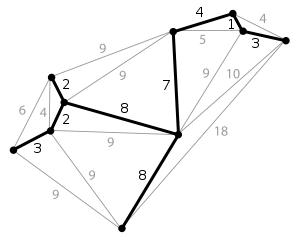
\includegraphics[width=0.3\textwidth]{minimum-spanning-tree}
          \caption{Ejemplo de \emph{Árbol Recubridor Mínimo}. (Extraido de \cite{wiki:Minimum_spanning_tree})}
          \label{img:minimum_spanning_tree}
        \end{figure}

        \paragraph{}
        La versión estática del problema del \emph{árbol recubridor mínimo} ha sido ampliamente estudiada en la literatura, existiendo un gran número de alternativas, entre las que destaca históricamente el \emph{Algoritmo de Kruskal} descrito en el artículo \emph{On the shortest spanning subtree of a graph and the traveling salesman problem} \cite{kruskal1956shortest} cuya complejidad temporal es de $O(n + log(m))$ sobre un espacio de $O(n+m)$.

        \paragraph{}
        También se han propuesto soluciones basadas en algoritmos probabilistas, que ofrecen garantias de optimalidad en su solución. La versión más eficiente encontrada hasta la fecha se describe en el trabajo \emph{An optimal minimum spanning tree algorithm} \cite{pettie2002optimal} de \emph{Pettie y otros}. Sin embargo, debido a las técnicas que utiliza (mediante reducción a \emph{Árboles de Decisión}) no se puede representar mediante una función, pero sí que se ha demostrado su optimalidad. El problema también se ha estudiado desde la perspectiva de la parelelización. En el trabajo \emph{Fast shared-memory algorithms for computing the minimum spanning forest of sparse graphs} \cite{bader2006fast} \emph{Bader y otros} muestran un algoritmo que mediante el multiprocesamiento consiguen soluciones $5$ veces más eficientes que la versión optimizada secuencial.

        \paragraph{}
        Una vez descrito el problema y su estado actual sobre el modelo estático, el resto del apartado se basará en la descripción del mismo sobre las restricciones del \emph{modelo en semi-streaming}. Para ello, se realiza una descripción del algoritmo exacto propuesto por \emph{Ahn y otros} en \emph{Analyzing graph structure via linear measurements} \cite{ahn2012analyzing}. Dicha estrategia es capaz de encontrar el \emph{árbol recubridor mínimo} en $O(log(n)/log(log(n)))$ pasadas sobre el stream de aristas ajustandose a las restricciones espaciales de $O(polylog(n))$.

        \paragraph{}
        El planteamiento del algoritmo en semi-streaming se basa inicialmente en el \emph{algoritmo de Boruvka’s} (en \cite{wiki:Boruvkas_algorithm} se encuentra una breve descripción), cuyo planteamiento es el siguiente: se realizan $O(log(n))$ de tal manera que en cada una de ellas se seleccionan las aristas de menor peso que conecten vértices aún no marcados como conectados. De manera incremental se construye el \emph{árbol recubridor mínimo} hasta que todos los vértices del grafo están conectados.

        \paragraph{}
        Tal y como se indica en el documento, el \emph{algoritmo de Boruvka’s} puede emularse fácilmente sobre el modelo en semi-streaming emulando cada fase en $O(log(n))$ pasadas por el stream (para encontrar el arista de menor peso), lo cual conlleva $O(log(log(n)))$ pasadas en total. La idea en que se basa el algoritmo para reducir el número de pasadas sobre el streaming es realizar la búsqueda del arista de menor peso de cada nodo en \say{paralelo}, teniendo en cuenta las limitaciones espaciales ($O(polylog(n))$) lo cual es posible en $O(log(n)/log(log(n)))$.


        \paragraph{}
        El problema del \emph{árbol recubridor mínimo} tiene aplicaciones prácticas en muchos entornos reales, como el diseño de redes de telecomunicaciones o de transporte. También se han encontrado reducciones sobre el \emph{Problema del Viajante} y el \emph{Problema del corte mínimo}. Otros usos son el análisis de estructuras de grafos, problemas de clustering o reconocimiento de estructuras sobre imágenes.

      \subsection{Componentes Conectados}
      \label{sec:graph_connected_components}

        \paragraph{}
        El problema de \emph{Componentes Conectados} se refiere a la búsqueda del cardinal de subconjuntos de vértices para los cuales existe un camino entre todos los vértices del subconjunto. Mediante este resultado se puede determinar por tanto si existe un camino que entre dos vértices simplemente comprobando si pertenecen al mismo subconjunto de componentes conectados. Nótese por tanto que un grafo conexo tan solo posee un único componente conectado que contiene todos los vértices del grafo.

        \paragraph{}
        Se denota como $cc(G)$ al cardinal de componentes conectados del grafo $G$. El algoritmo clásico para resolver este problema se describe a continuación. Este requiere de $O(log(n))$ fases para su finalización y se basa en la fusión de vértices conectados. En cada fase se fusiona cada vértice con otro que posea una arista incidente a el para después crear un \emph{super-vértice} con el cual se relacionen las aristas de los dos vértices fusionados. Tras realizar esta operación repetidas veces, el algoritmo termina cuando ya no es posible fusionar mas vértices. El número de \emph{super-vértices} resultantes, por tanto es equivalente a $cc(G)$.

        \paragraph{}
        En el trabajo \emph{Analyzing graph structure via linear measurements} \cite{ahn2012analyzing} se describe un algoritmo para realizar dicha tarea sobre el \emph{modelo en semi-streaming} en una única pasada y con una complejidad espacial de $O(n \cdot log(n))$. Para ello, se basa en la construcción de sketches a partir del \emph{$L_0$-Samplers} denotados como $S_1, S_2, ..., S_t$ con $t = O(log(n))$. Esto conlleva un coste espacial de $O(n\cdot t \cdot log(log(n)))$, por lo que es válido sobre el \emph{modelo en semi-streaming}. La idea es la construcción jerárquica de estos sketches, de tal manera que $S_1$ represente el sketch de las aristas de los vértices del grafo $G$, $S_2$ las aristas de los \emph{super-vértices} generados en la primera iteracción, y así sucesivamente, de tal manera que a partir de $S_t$ se puede obtener $cc(G)$ al igual que en el algoritmo básico.

        \paragraph{}
        En \cite{ahn2012analyzing}, además, se extiende dicho algoritmo para el problema de \emph{$k$-aristas conectadas}, que indica el número mínimo de aristas incidentes sobre cada vértice. Las aplicaciones prácticas tanto de este problema como el de \emph{componentes conectados} son de utilizad para conocer la estructura del grafo. Un ejemplo práctico se da en grafos referidos a redes sociales, en las cuales se pretende encontrar el número de agrupaciones (o \emph{clusters}) de usuarios aislados del resto, así como el número mínimo de amistades que presenta cada usuario.

      \subsection{Paseos Aleatorios}
      \label{sec:random_walks_overview}

        \paragraph{}
        Un paseo aleatorio se define como la distribución de probabilidad referida a la realización de un camino de longitud $l$ desde un determinado vértice de inicio fijado \emph{a-priori}. Suponiendo que en cada vértice se tiene una distribución de probabilidad sobre sus aristas incidentes, entonces este problema está intimamente relacionado con las \emph{cadenas de Markov}.

        \paragraph{}
        El algoritmo PageRank se refiere a la obtención del estado estacionario de la distribución de probabilidad de los paseos aleatorios con algunas modificaciones. Tanto los \emph{paseos aleatorios} como las cadenas de Markov se describen en detalle en el capítulo \ref{chap:pagerank} destinado al algoritmo PageRank.

    \section{Conclusiones}
    \label{sec:graph_conclusions}

      \paragraph{}
      A lo largo del capítulo se han citado distintas estrategias mediante las cuales se pretende reducir el grado de complejidad para la resolución de problemas sobre grafos, lo cual implica una reducción del tiempo de computo y del espacio necesario. Estas técnicas están ganando una gran relevancia en la actualidad debido a la necesidad de obtener respuestas en un periodo corto de tiempo, lo cual permite mejorar la toma de decisiones.

      \paragraph{}
      Debido al dinamismo del entorno en que vivimos en un gran número de ocasiones es más beneficioso encontrar soluciones aproximadas que no otorgan el rendimiento óptimo, pero que son obtenidas en un tiempo mucho menor, lo cual permite una rápida adaptación a cambios. Mediante este punto de vista, se pueden obtener mayores beneficios en promedio, puesto que los sobrecostes temporales propiciados por el tiempo de respuesta en soluciones exactas muchas veces conllevan que estos queden obsoletos rápidamente.

      \paragraph{}
      Se cree que en los próximos años, el estudio e investigación en el ámbito de la resolución de problemas sobre grafos de tamaño masivo será creciente, al igual que sucedia en el caso numérico como se indicó en anteriores capítulos. A pesar de ello, debido a su mayor grado de dificultad, dichos avances son lentos y actualmente se encuentran en fases muy tempranas de desarrollo, pero tal y como se ha indicado, se espera que esta situación cambie en el futuro.

\end{document}
